%\documentclass{article}
%\usepackage{graphicx,subfigure}
%\begin{document}

\begin{figure}[!h]
  \centering
   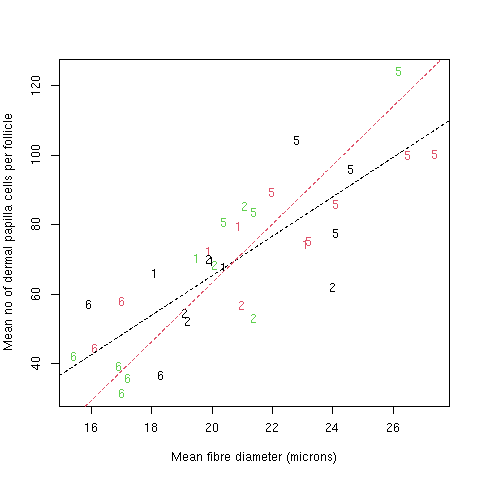
\includegraphics[width=0.9\textwidth]{dpccdiam2.png}
  \caption{Plot of mean fibre diameter against mean number of dermal papilla cells per follicle for 34 sheep from CSIRO selection experiments. The coloured numbers representing each point indicate the selection line (1 = high staple length, 2 = low staple length, 5 = high fibre diameter, 6 = low fibre diameter). The two dashed lines are   linear regressions of papilla cell count on diameter (black) and of diameter on papilla cell count (red).}
  \label{fig:dpccdiam}
\end{figure}

%\end{document}

